\documentclass{article}
\usepackage[spanish]{babel}
\usepackage[utf8]{inputenc}
\usepackage{amsmath}
\usepackage{graphicx}
\usepackage{hyperref}
\usepackage{float}

\title{Estrategia para el Juego Hex}
\author{Claudia Hernández Pérez \\ C-312}
\date{\today}

\begin{document}

\maketitle

\vspace{2cm}

\begin{figure}[h]
    \centering
    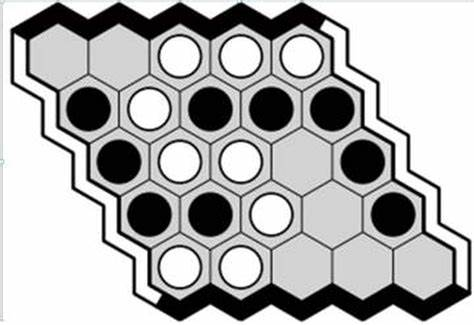
\includegraphics[width=5cm]{./images/hex_board.jpg}
\end{figure}

\newpage

\section{Visión General}
La estrategia implementada combina tres técnicas principales: \textbf{Monte Carlo Tree Search (MCTS)}, \textbf{Minimax con poda alfa-beta}, y una \textbf{heurística basada en A*}. La elección entre métodos depende de la fase de la partida, priorizando eficiencia y profundidad según la complejidad del tablero.

\section{Componentes Clave}

\subsection{Movimiento Inicial: Ocupar el Centro}
\begin{itemize}
\item \textbf{Lógica}: Si el centro del tablero está libre, se juega allí.
\item \textbf{Objetivo}: Controlar una posición estratégica que facilita conexiones en múltiples direcciones.
\end{itemize}

\subsection{Chequeo Táctico: Victoria o Bloqueo Inmediato}
\begin{itemize}
\item \textbf{Lógica}: Verifica si existe un movimiento que gane la partida o bloquee una victoria inmediata del rival.
\item \textbf{Objetivo}: Si tengo una victoria clara en un movimiento se juega allí, si por el contrario mi oponente es quien
    gana en un movimiento lo obstaculizo.
\end{itemize}

\subsection{Selección de Estrategia según Fase de la Partida}

\subsubsection{Fase Temprana (muchas celdas vacías)}
\begin{itemize}
\item \textbf{Algoritmo}: Monte Carlo Tree Search (MCTS) con profundidad limitada.
\item \textbf{Objetivo}: Explorar eficientemente movimientos prometedores.
\item \textbf{Detalles}:
\begin{itemize}
\item Realiza 1000 simulaciones aleatorias por movimiento.
\item Evalúa resultados con función heurística basada en A*.
\end{itemize}
\end{itemize}

\subsubsection{Fase Tardía (menos celdas vacías)}
\begin{itemize}
\item \textbf{Algoritmo}: Minimax con poda alfa-beta y profundidad adaptativa.
\item \textbf{Objetivo}: Analizar secuencias de movimientos en profundidad.
\item \textbf{Detalles}:
\begin{itemize}
\item La profundidad (\texttt{depth}) aumenta conforme avanza la partida.
\item Usa poda alfa-beta para reducir cálculos.
\end{itemize}
\end{itemize}

\subsection{Minimax con Poda Alfa-Beta}
\begin{itemize}
\item \textbf{Funcionamiento}:
\begin{itemize}
\item \textbf{Maximizador}: Busca maximizar la evaluación para el jugador actual.
\item \textbf{Minimizador}: Simula jugadas del rival para minimizar la evaluación.
\end{itemize}
\item \textbf{Profundidad Adaptativa}:
\[ \text{depth} = \left\lfloor \frac{\text{board.size}^2}{\text{board.size}^2 - 2 \times \text{rounds}} \right\rfloor + 1 \]
\item \textbf{Explicación}: Por cada ronda se juegan dos posiciones (2 * rounds) y el total de casillas es $\text{board.size}^2$,
    a medida que avance el juego habrán menos casillas lo que me permitirá reemplazar esfuerzos de casillas en profundidad.
\end{itemize}

\subsection{Heurística basada en A* (HSearch)}
\begin{itemize}
\item \textbf{Objetivo}: Evaluar la facilidad de conectar los lados del jugador.
\item \textbf{Métricas}:
\begin{itemize}
\item \textbf{Costo del Jugador}: Esfuerzo mínimo para conectar sus lados.
\item \textbf{Costo del Rival}: Esfuerzo mínimo del adversario.
\end{itemize}
\item \textbf{Función de Evaluación}:
\[ \text{eval} = \frac{1}{\text{my\_cost}} + \text{opp\_cost} \]
\item \textbf{Explicación}: La mejor evaluación de esta función será cuando al jugador le queden menos piezas para ganar y 
    cuando más le queden al oponente.
\end{itemize}

\section{Flujo de Decisión}
\begin{enumerate}
\item \textbf{Movimiento Inicial}: Ocupar el centro si está libre.
\item \textbf{Chequeo Táctico}: Jugar movimiento ganador o bloqueo si existe.
\item \textbf{Estrategia Principal}:
\begin{itemize}
\item Fase Temprana: MCTS con simulaciones rápidas.
\item Fase Tardía: Minimax con búsqueda profunda.
\end{itemize}
\item \textbf{Evaluación Heurística}: Usar A* para comparar posiciones.
\end{enumerate}

\section{Fortalezas}
\begin{itemize}
\item \textbf{Adaptabilidad}: Cambia entre métodos según la fase de la partida.
\item \textbf{Eficiencia}: Poda alfa-beta y MCTS reducen el espacio de búsqueda.
\item \textbf{Tácticas Inmediatas}: Detecta victorias/bloqueos en 1 movimiento (potencial optimización temporal).
\end{itemize}

\end{document}